\section{代理模型}
\label{sec:ns-surrogate}

光滑化一开始就把目标换掉，此后只和替代函数打交道。本节考虑另一种做法：目标不换，每一轮在当前点围绕它造一个容易求解的\term{代理模型}（surrogate model），用模型的解作为候选更新。问题是：模型什么时候能代表原目标取得进展？

模型易解并不说明什么，关键是模型和原目标是什么关系。第~\ref{sec:ns-mm}小节的模型处处在原目标上方，解了就直接下降。第~\ref{sec:ns-bundle}小节的模型处处在下方，只能预测，候选点要回到原目标上检验。

\subsection{MM方法}
\label{sec:ns-mm}

回顾邻近梯度法。式~\eqref{eq:ns-composite-model}的模型在$\alpha\leq1/L$时处处不低于$F$，在当前点与$F$相等，而模型的最小点至少不高于当前值，这三条保证了下降。把这三条抽出来，就不必是二次上界了。

\begin{definition}[上界代理与MM更新]
\label{def:ns-mm}
设$F:\mathbb{R}^n\to\mathbb{R}\cup\{+\infty\}$，$\bm{x}^{(t)}\in\operatorname{dom}F$。函数$Q(\cdot\mid\bm{x}^{(t)})$若满足
\begin{gather}
 Q(\bm{x}\mid\bm{x}^{(t)})\geq F(\bm{x})\qquad\text{对所有}\ \bm{x},\label{eq:ns-mm-majorize}\\
 Q(\bm{x}^{(t)}\mid\bm{x}^{(t)})=F(\bm{x}^{(t)}),\label{eq:ns-mm-touch}
\end{gather}
就称为$F$在$\bm{x}^{(t)}$处的\term{上界代理}（majorizer）。选取满足下式的新点，
\begin{equation}
 Q(\bm{x}^{(t+1)}\mid\bm{x}^{(t)})\leq Q(\bm{x}^{(t)}\mid\bm{x}^{(t)}),
 \label{eq:ns-mm-progress}
\end{equation}
这样的迭代称为\term{MM方法}（majorization-minimization）。
\end{definition}

三项要求合起来给出一串不等式：
\begin{equation}
 F(\bm{x}^{(t+1)})\leq Q(\bm{x}^{(t+1)}\mid\bm{x}^{(t)})\leq Q(\bm{x}^{(t)}\mid\bm{x}^{(t)})=F(\bm{x}^{(t)}).
 \label{eq:ns-mm-chain}
\end{equation}

第一步用上界，第二步用子问题的进展，第三步用接触。所以不需要精确地求最小点，只需要代理值不升。$F$不要求凸，也不要求可微。式~\eqref{eq:ns-mm-chain}的三处都不能少：若只有$\bm{x}^{(t)}$附近上界成立，第一步在远处就失败，候选点要限制在有效区域内；若模型只在当前点相切而不高于$F$，比如凸函数的切线，第一步方向就反了。

可以把上界代理想成在地形上方铺一块柔软的毯子，毯子在脚下贴住地面。把毯子的最低点作为下一步，地面只会比毯子更低，脚下的地面就下降了。

\paragraph{例：绝对值和的二次上界}
要最小化$F(x)=\sum_i\lvert x-y_i\rvert$，也就是求中位数。把每个绝对值换成二次上界。对$c\neq0$，由$(\lvert r\rvert-\lvert c\rvert)^2\geq0$，
\begin{equation}
 \lvert r\rvert\leq\frac{r^2}{2\lvert c\rvert}+\frac{\lvert c\rvert}{2},
 \label{eq:ns-abs-majorizer}
\end{equation}
并且$r=\pm c$时取等号。对每一项取$c=x^{(t)}-y_i$，得到代理
\[
 Q(x\mid x^{(t)})=\sum_i\Bigl(\frac{(x-y_i)^2}{2\lvert x^{(t)}-y_i\rvert}+\frac{\lvert x^{(t)}-y_i\rvert}{2}\Bigr).
\]

代理是二次函数，最小点是加权平均：
\begin{equation}
 x^{(t+1)}=\frac{\sum_iw_iy_i}{\sum_iw_i},\qquad w_i=\frac{1}{\lvert x^{(t)}-y_i\rvert}.
 \label{eq:ns-irls}
\end{equation}

这种由当前残差定权重、解加权最小二乘的方法称为\term{迭代重加权最小二乘}（iteratively reweighted least squares，IRLS）。

用数据$y=(0,1,5)$，从$x^{(0)}=3$开始。此时$F(3)=7$，三个权重是$(\tfrac13,\tfrac12,\tfrac12)$，由式~\eqref{eq:ns-irls}，
\[
 x^{(1)}=\frac{0+\tfrac12+\tfrac52}{\tfrac43}=\frac94,\qquad F(x^{(1)})=6.25.
\]

第二轮的权重变成$(\tfrac49,\tfrac45,\tfrac{4}{11})$，
\[
 x^{(2)}\approx1.628,\qquad F(x^{(2)})\approx5.628.
\]

继续下去依次是$x^{(3)}\approx1.229$和$x^{(4)}\approx1.045$，$F$逐轮降到最优值$5$，最优解是中位数$1$。靠近中位数的数据点权重越来越大，第四轮权重已经约为$22$，这正是非光滑的尖点在代理里的反映。

\begin{BookInlineFigure}
  \centering
  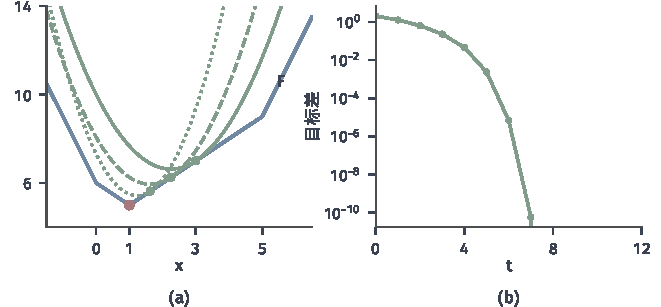
\includegraphics[width=112mm]{figures/05-optimization/03-nonsmooth-optimization/matplotlib/ns-mm-surrogates/figure.pdf}
  \caption{中位数问题的MM迭代，$F(x)=\lvert x\rvert+\lvert x-1\rvert+\lvert x-5\rvert$，$x^{(0)}=3$。(a)蓝线是$F$，绿色实线、虚线、点线是前三轮的二次代理，绿点是接触点，红点是最优解。(b)目标差（对数坐标）逐轮下降。}
  \label{fig:ns-mm-surrogates}
\end{BookInlineFigure}

图~\ref{fig:ns-mm-surrogates}(a)显示每条代理都贴住当前点，并处处在$F$上方。这里也有一个需要小心的地方：当前点若恰好落在某个$y_i$上，$c=0$，式~\eqref{eq:ns-abs-majorizer}没有定义。常用的修正把权重改成$1/\max\{\lvert x^{(t)}-y_i\rvert,\delta\}$。容易误解的是，修正后的代理不再是$\lvert r\rvert$的上界，而是Huber函数$h_\delta(r)$的上界：函数$s\mapsto h_\delta(\sqrt{s})$对$s\geq0$是凹的，取切线就得到这个权重。所以修正后的迭代求解的是第~\ref{sec:ns-huber}小节的替代目标，这时需要按第~\ref{sec:ns-smoothing-accuracy}小节计入偏差。

\paragraph{目标下降与收敛到最优解的区别}
式~\eqref{eq:ns-mm-chain}只说目标值不增。$F$有下界时目标值序列收敛，但它收敛到什么地方，要看$F$本身。

用一个非凸的稀疏罚函数说明。设
\begin{equation}
 F(x)=\frac12(x-3)^2+\frac72\ln(1+\lvert x\rvert).
 \label{eq:ns-reweighted-example}
\end{equation}

函数$s\mapsto\ln(1+s)$在$s\geq0$上是凹的，所以在当前点取切线就是上界。把$\ln(1+\lvert x\rvert)$换成这个上界，代理为
\[
 Q(x\mid c)=\frac12(x-3)^2+\frac72\Bigl(\ln(1+\lvert c\rvert)+\frac{\lvert x\rvert-\lvert c\rvert}{1+\lvert c\rvert}\Bigr).
\]

代理是一个带绝对值的二次函数，最小点由软阈值给出：
\begin{equation}
 x^{(t+1)}=S_{\tau^{(t)}}(3),\qquad\tau^{(t)}=\frac{7/2}{1+\lvert x^{(t)}\rvert}.
 \label{eq:ns-reweighted-update}
\end{equation}

从$x^{(0)}=1$出发，阈值依次是$1.75$，$1.556$，$1.432$，序列是
\[
 1,\ \ 1.25,\ \ 1.444,\ \ 1.568,\ \ldots\to1+\frac{\sqrt2}{2}\approx1.707,
\]
目标值从$4.426$单调下降到约$4.321$。从$x^{(0)}=0.2$出发，阈值是$2.917$，$3.231$，序列是
\[
 0.2,\ \ 0.083,\ \ 0,\ \ 0,\ \ldots
\]
目标值从$4.558$单调下降到$4.5$，然后停住。$x=0$是一个局部最小点：$F$在此处的右导数是$-3+3.5>0$，左导数是$-3-3.5<0$，代理的阈值$3.5$也比数据$3$大。

两条序列都满足不等式链，一条到达全局最优值$4.321$，另一条停在$4.5$。图~\ref{fig:ns-mm-reweighted}显示了这两个吸引域。

\begin{BookInlineFigure}
  \centering
  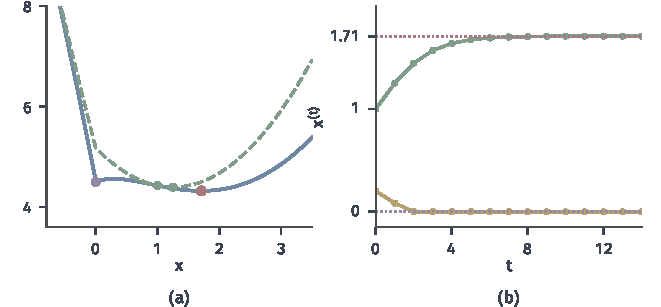
\includegraphics[width=112mm]{figures/05-optimization/03-nonsmooth-optimization/matplotlib/ns-mm-reweighted/figure.pdf}
  \caption{MM在非凸目标上的两个结局，目标是式~\eqref{eq:ns-reweighted-example}。(a)蓝线是$F$，绿色虚线是$x=1$处的代理，绿点是接触点和代理的最小点。红点是全局最优解，紫点是另一个局部最优解$x=0$。(b)迭代序列，绿线从$1$出发到全局最优解，黄线从$0.2$出发停在局部最优解。}
  \label{fig:ns-mm-reweighted}
\end{BookInlineFigure}

要把目标值收敛提升到“极限点是驻点”，还需要额外的条件：常见的要求是代理与原目标在接触点的方向导数一致，代理随当前点连续变化，子问题的解足够接近代理的最小点。要说全局最优，还得有凸性。MM的优点是简单和单调，没有给出离最优值还有多远。

\subsection{束方法}
\label{sec:ns-bundle}

次梯度法每步用一条支撑线，用完就丢了。对凸目标，每一条支撑线都是全局的下界，丢掉很可惜。\term{束方法}（bundle method）把读到的支撑线都留下，拼成一个下界模型。

\paragraph{主要思想}
设$f:\mathbb{R}^n\to\mathbb{R}$是凸函数，读取程序在点$\bm{y}$返回函数值和一个次梯度。假设已经在$\bm{y}^{(0)},\ldots,\bm{y}^{(t)}$处读到次梯度$\bm{g}_0,\ldots,\bm{g}_t$，由支撑不等式，
\begin{equation}
 m^{(t)}(\bm{x})=\max_{0\leq j\leq t}\bigl\{f(\bm{y}^{(j)})+\langle\bm{g}_j,\bm{x}-\bm{y}^{(j)}\rangle\bigr\}\leq f(\bm{x}).
 \label{eq:ns-cutting-plane}
\end{equation}

这个分段线性模型称为\term{割平面模型}（cutting-plane model），读到的这一组支撑线合称束。它在读过的点上等于$f$，别处低估$f$。

直接最小化$m^{(t)}$不行。开始时模型只有一条直线，根本没有最小点；后面它的最小点也可能远远地落在信息不足的地方。解决办法是设一个\term{稳定中心}（stability center）$\hat{\bm{x}}^{(t)}$，表示目前已确认的好点，加一个距离项把候选点拉在中心附近：
\begin{equation}
 \bm{y}^{(t+1)}=\argmin_{\bm{x}}\Bigl\{m^{(t)}(\bm{x})+\frac{1}{2\tau}\lVert\bm{x}-\hat{\bm{x}}^{(t)}\rVert_2^2\Bigr\},\qquad\tau>0.
 \label{eq:ns-bundle-candidate}
\end{equation}

这是模型的邻近映射$\operatorname{prox}_{\tau m^{(t)}}(\hat{\bm{x}}^{(t)})$，解存在且唯一。引入变量$v$表示模型值，子问题是一个小的二次规划：最小化$v+\lVert\bm{x}-\hat{\bm{x}}^{(t)}\rVert_2^2/(2\tau)$，约束是$v$不低于束中每条支撑线在$\bm{x}$处的值。

\paragraph{接受还是拒绝}
模型预测下降
\begin{equation}
 \delta^{(t)}=f(\hat{\bm{x}}^{(t)})-m^{(t)}(\bm{y}^{(t+1)}).
 \label{eq:ns-predicted-decrease}
\end{equation}

因为子问题在$\hat{\bm{x}}^{(t)}$处的值就是$f(\hat{\bm{x}}^{(t)})$（中心处的支撑线在束内），而$\bm{y}^{(t+1)}$是子问题的最小点，所以$\delta^{(t)}\geq0$。但模型是下界，预测往往偏乐观，必须用原目标检验。给定$\beta\in(0,1)$，判断
\begin{equation}
 f(\hat{\bm{x}}^{(t)})-f(\bm{y}^{(t+1)})\geq\beta\,\delta^{(t)}.
 \label{eq:ns-serious-test}
\end{equation}

式~\eqref{eq:ns-serious-test}成立就把中心移到候选点，称为\term{实质步}（serious step）；否则中心不动，称为\term{空步}（null step）。两种情况都把$\bm{y}^{(t+1)}$处的新支撑线加入束。

实质步是有效的移动，空步是对模型的改进。空步没有白费，它恰好在模型低估最严重的地方补上一条割线，下一次预测就准了。这是束方法和前面的方法的一个显著差别：不是每一步都移动，但每一步都学到东西。

\paragraph{计算过程}
用三段折线$f(x)=\max\{-x,x/2,2x-3\}$，$\tau=2$，$\beta=\tfrac12$。

\needspace{6\baselineskip}
\paragraph{变量}
\begin{itemize}
 \item 束：列表$\{(\bm{y}^{(j)},f(\bm{y}^{(j)}),\bm{g}_j)\}$。
 \item $\hat{\bm{x}}^{(t)}$：稳定中心；$\delta^{(t)}$：预测下降。
 \item $\tau$，$\beta$，容差$\varepsilon$。
\end{itemize}

\paragraph{初始化}
选$\bm{y}^{(0)}$，读取$f$和一个次梯度，令$\hat{\bm{x}}^{(0)}=\bm{y}^{(0)}$。例中$y^{(0)}=4$，$f(4)=5$，$g_0=2$。

\needspace{6\baselineskip}
\paragraph{每轮更新}
\begin{enumerate}
 \item 由式~\eqref{eq:ns-bundle-candidate}解候选点。例中第一轮模型只有一条直线，
 \[
  m^{(0)}(x)=2x-3,\qquad y^{(1)}=4-2\tau=0.
 \]
 \item 由式~\eqref{eq:ns-predicted-decrease}算预测下降；若$\delta^{(t)}\leq\varepsilon$，停止，返回$\hat{\bm{x}}^{(t)}$。例中第一轮
 \[
  \delta^{(0)}=5-(-3)=8.
 \]
 \item 读取$f(\bm{y}^{(t+1)})$和次梯度，加入束。例中第一轮
 \[
  f(0)=0,\qquad g_1=\frac12.
 \]
 \item 由式~\eqref{eq:ns-serious-test}决定是否移动中心。例中第一轮实际下降是$5\geq\tfrac12\cdot8$，实质步，中心移到$0$。
\end{enumerate}

第二轮的模型多了一条直线，$m^{(1)}(x)=\max\{2x-3,\ x/2\}$。中心在$0$，子问题的解在$x/2$这一支上，令$\tfrac12+x/2=0$，得到
\[
 y^{(2)}=-1,\qquad m^{(1)}(-1)=-\frac12,\qquad\delta^{(1)}=\frac12.
\]

实际$f(-1)=1$，比中心$f(0)=0$还高，实际下降是$-1$，小于$\beta\delta^{(1)}=\tfrac14$，是空步，中心不动。把$x=-1$处斜率$-1$的支撑线$-x$加入束。

第三轮模型变成$\max\{2x-3,\ x/2,\ -x\}$，在中心$0$的次微分是$[-1,\tfrac12]$，包含$0$，所以$y^{(3)}=0$，
\[
 \delta^{(2)}=0.
\]

预测下降为零，停止，最终得到$\hat{x}=0$，也就是最优解。图~\ref{fig:ns-bundle-1d}逐轮画出了模型：(b)的模型过分乐观，(c)补上割线后预测就准了。

\begin{BookInlineFigure}
  \centering
  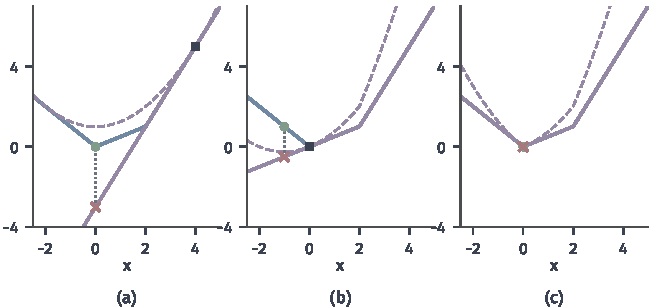
\includegraphics[width=112mm]{figures/05-optimization/03-nonsmooth-optimization/matplotlib/ns-bundle-1d/figure.pdf}
  \caption{束方法在三段折线上的三轮，$\tau=2$。蓝线是$f$，紫色实线是割平面模型，紫色虚线是模型加距离项，黑方块是稳定中心。红叉是候选点处的模型值，绿点是候选点处的真实目标值。(a)第一轮，实质步。(b)第二轮，候选点$-1$处模型偏低，真实目标值反而高，空步。(c)第三轮，候选点就是中心，预测下降为零，停止。}
  \label{fig:ns-bundle-1d}
\end{BookInlineFigure}

\paragraph{评价原目标的误差}
预测下降$\delta^{(t)}$既用于接受判断，也是一个停止证书。子问题的最优性条件给出
\[
 \bm{s}^{(t)}=\frac{\hat{\bm{x}}^{(t)}-\bm{y}^{(t+1)}}{\tau}\in\partial m^{(t)}(\bm{y}^{(t+1)}).
\]

由模型是$f$的下界和$\bm{s}^{(t)}$是模型的次梯度，对任意$\bm{x}$，
\[
 f(\bm{x})\geq m^{(t)}(\bm{x})\geq m^{(t)}(\bm{y}^{(t+1)})+\langle\bm{s}^{(t)},\bm{x}-\bm{y}^{(t+1)}\rangle.
\]

由式~\eqref{eq:ns-predicted-decrease}替换模型值，再用$\bm{s}^{(t)}$的定义把候选点写成$\hat{\bm{x}}^{(t)}$减$\tau\bm{s}^{(t)}$，整理后得到
\begin{equation}
 f(\bm{x})\geq f(\hat{\bm{x}}^{(t)})+\langle\bm{s}^{(t)},\bm{x}-\hat{\bm{x}}^{(t)}\rangle-e^{(t)},\qquad e^{(t)}=\delta^{(t)}-\tau\lVert\bm{s}^{(t)}\rVert_2^2.
 \label{eq:ns-bundle-certificate}
\end{equation}

取$\bm{x}=\hat{\bm{x}}^{(t)}$得$e^{(t)}\geq0$，所以$\tau\lVert\bm{s}^{(t)}\rVert_2^2\leq\delta^{(t)}$，$e^{(t)}\leq\delta^{(t)}$。式~\eqref{eq:ns-bundle-certificate}说$\bm{s}^{(t)}$是一个带误差$e^{(t)}$的近似次梯度。设中心到某个最优解的距离不超过$R$，在式中取$\bm{x}=\bm{x}^\star$，得到
\begin{equation}
 f(\hat{\bm{x}}^{(t)})-f^\star\leq e^{(t)}+R\lVert\bm{s}^{(t)}\rVert_2\leq\delta^{(t)}+R\sqrt{\frac{\delta^{(t)}}{\tau}}.
 \label{eq:ns-bundle-error}
\end{equation}

这个界每一轮都可以直接计算，不需要任何收敛定理。例中第三轮$\delta^{(2)}=0$，$\bm{s}^{(2)}=0$，这一轮的证书说明误差为零。

\paragraph{收敛与成本}
在凸目标、次梯度有界的条件下，邻近束方法的中心目标值收敛到$f^\star$，实质步无穷多和有限多两种情形要分别讨论，证明篇幅较长。这里强调它的成本结构。

图~\ref{fig:ns-bundle-2d}在平面上比较束方法与次梯度法，横轴是原目标的读取次数。束方法只用很少几次读取就到达很高的精度，这得益于分段线性目标正好是割平面模型的同类，代价是每轮要解一个二次规划，约束个数随束增长。实践中会合并或丢弃不活跃的割线，这需要额外的规则来保证模型仍然有效。

\begin{BookInlineFigure}
  \centering
  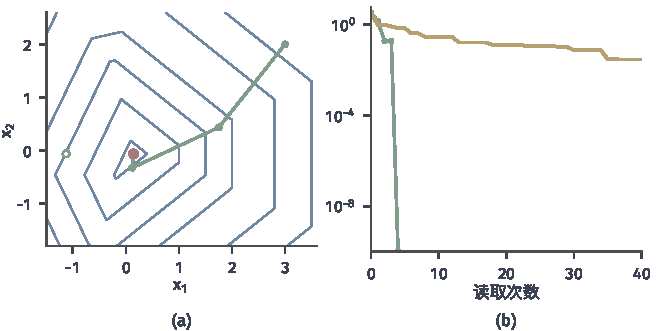
\includegraphics[width=112mm]{figures/05-optimization/03-nonsmooth-optimization/matplotlib/ns-bundle-2d/figure.pdf}
  \caption{束方法与次梯度法，目标与图~\ref{fig:ns-smoothing-budget}相同，$\bm{x}^{(0)}=(3,2)$。(a)蓝线是等高线，红点是最优解，绿色实心点和折线是实质步，空心圆是空步的候选点。(b)绿线是束方法的中心目标差，黄线是次梯度法的最好目标差（步长$\sqrt{13}/\sqrt{t+1}$），横轴是原函数读取次数，纵轴为对数坐标。}
  \label{fig:ns-bundle-2d}
\end{BookInlineFigure}

\paragraph{上界模型与下界模型}
两种模型提供的信息不同，表~\ref{tab:ns-surrogates}把它们和前面的光滑化放在一起比较。上界模型给出保证而无需再读原目标，但不告诉离最优有多远。下界模型给出离最优的证书，但每步都要检验。把下界模型的解直接当作进展，或者把上界模型的最小值当作下界，都是错误的用法。

\begin{BookInlineTable}
  \centering
  \small
  \begin{tabular}{@{}llll@{}}
    \toprule
     & MM & 束方法 & 光滑化\\
    \midrule
    辅助函数 & 上界，每轮重建 & 下界，逐轮累加 & 固定的光滑替代\\
    与原目标的关系 & 处处在上方 & 处处在下方 & 相差不超过$\mu D$\\
    接受规则 & 代理值不增 & 实际下降够大 & 无\\
    原目标逐轮 & 不增 & 中心不增 & 可以上升\\
    误差证书 & 无 & 式~\eqref{eq:ns-bundle-error} & 式~\eqref{eq:ns-smoothing-split}\\
    主要成本 & 代理子问题 & 二次规划 & 梯度次数\\
    \bottomrule
  \end{tabular}
  \caption{三种辅助模型的对照。}
  \label{tab:ns-surrogates}
\end{BookInlineTable}
